\chapter[Estado del arte y tecnologías utilizadas]{Estado del arte y tecnologías utilizadas}
\chaptermark{Arte y tecnologías}
\label{chap:estado del arte}

\section[Estado del arte de herramientas para monitorizar información]{Estado del arte de herramientas para monitorizar información}
\sectionmark{Estado del arte}


%\newpage
\section{Tecnologías utilizadas}

A continuación se detallan las diferentes tecnologías/bibliotecas/lenguajes que se han empleado para la elaboración del proyecto y por qué se han escogido por encima de otras posibles soluciones.


\subsection{\LaTeX}

Web: \url{https://www.latex-project.org/}\\

\LaTeX es un lenguaje de marcado que sirve para la redacción de documentos científicos o técnicos. Con esta herramienta o lenguaje se ha desarrollado la memoria actual del proyecto de final de carrera.



\subsection{WebStorm}

\hspace*{2.25in}{
\includegraphics[scale=0.25]{imagenes/webstorm-logo.png}}

Web: \url{https://www.jetbrains.com/webstorm/}\\

WebStorm es un IDE de JavaScript ligero pero potente, perfectamente equipado para el desarrollo del lado del cliente y el desarrollo del servidor con Node.js. Permite la integración con frameworks de desarollo como Sails js. Para el desarrollo de la aplicación se optó por este IDE. \\

\subsection{Github}


\hspace*{2.25in}{
\includegraphics[scale=0.25]{imagenes/github-logo.png}}

Web: \url{https://about.github.com/}\\
Repositorio: \url{https://github.com/lopi87/SAILS-RobotUI}\\


GitHub es una forja (plataforma de desarrollo colaborativo) para alojar proyectos utilizando el sistema de control de versiones Git. Utiliza el framework Ruby on Rails por GitHub, Inc. (anteriormente conocida como Logical Awesome). Desde enero de 2010, GitHub opera bajo el nombre de GitHub, Inc. El código se almacena de forma pública, aunque también se puede hacer de forma privada, creando una cuenta de pago.


\subsection{Git}

\hspace*{2.1in}{
\includegraphics[scale=0.5]{imagenes/git-logo.png}}

Web: \url{https://git-scm.com/}\\

Git es un sistema open-source de control de versiones diseñado para manejar integramente las fases de desarrollo de proyectos, simples y complejos, con velocidad y eficiencia.\\

\subsection{Digital Ocean}

\begin{center}
\includegraphics[scale=0.35]{imagenes/docean-logo.png}\end{center}

Web: \url{https://www.digitalocean.com/}\\

Servidor web para alojar proyectos en la nube. La ventaja de este servicio de VPS es que te permite desplegar máquinas de cualquier tipo (siempre que sean software libre) de una manera muy fácil y rápida. Además tiene un punto fuerte y es que la información se almacena en discos SSD, con lo que el procesamiento se ve muy mejorado a la hora de computar (en este caso trabajo con web sockets y transmisión de datos).\\

\begin{figure}[H]
\begin{center}
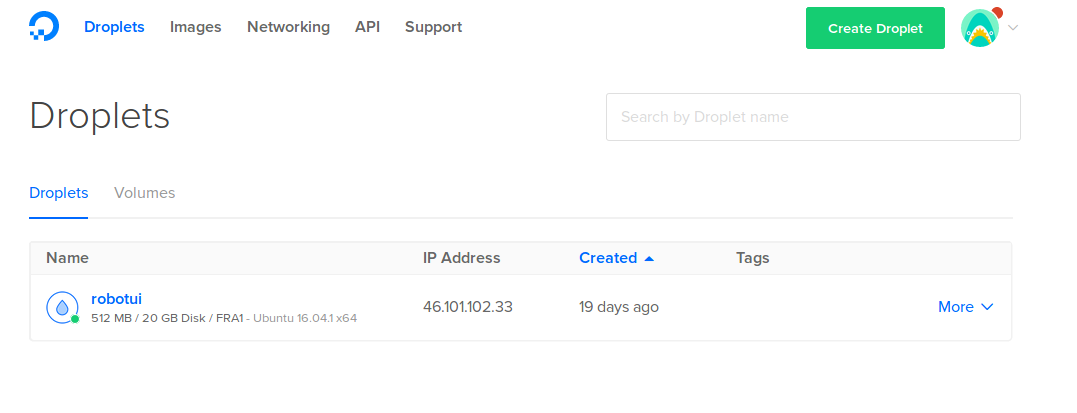
\includegraphics[scale=0.45]{imagenes/droplets.png}
\caption{Droplet desplegado en digital ocean}
\end{center}
\end{figure}


\subsection{Node js}

\begin{center}

\includegraphics[scale=0.3]{imagenes/nodejs-logo.png}
\end{center}

Web: \url{https://nodejs.org/es/}\\

Node.js es un entorno de ejecución para JavaScript construido con el motor de JavaScript V8 de Chrome. Node.js usa un modelo de operaciones E/S sin bloqueo y orientado a eventos, que lo hace liviano y eficiente. Incorpora un sistema de gestión de paquetes llamado, npm, es el ecosistema mas grande de librerías de código abierto en el mundo.\\

Node.js tiene una arquitectura basada en eventos capaz de E/S asíncronos. Estas opciones de diseño apuntan a optimizar el rendimiento y la escalabilidad en aplicaciones Web con muchas operaciones de entrada/salida, así como para aplicaciones Web en tiempo real (por ejemplo, programas de comunicación en tiempo real y juegos de navegador), lo que lo hacen ideal para este proyecto.\\


\subsection{Sails js}

\begin{center}

\includegraphics[scale=0.5]{imagenes/sailsjs-logo.png}
\end{center}

Web: \url{http://sailsjs.com/}\\

Sails.js es un framework web que facilita la creación de aplicaciones personalizadas Node.js de nivel empresarial. Está diseñado para parecerse a la arquitectura MVC de frameworks como Ruby on Rails, pero con soporte para el estilo de desarrollo de aplicaciones web más moderno y orientado a datos.\\

Utiliza Express para funciones como la gestión de peticiones HTTP y websockets. Su envoltorio intuitivo de websockets lo hace especialmente bueno para construir características en tiempo real como por ejemplo un Chat, por estas razones se ha considerado como el framework más adecuado hasta la fecha para la elaboración de este proyecto.

\subsection{Socket io}




\subsection{Bootstrap}


\begin{center}

\includegraphics[scale=0.3]{imagenes/bootstrap-logo.jpg}
\end{center}

Web: \url{http://getbootstrap.com/}\\

Bootstrap es un framework o conjunto de herramientas de Código abierto para diseño de sitios y aplicaciones web. Contiene plantillas de diseño con tipografía, formularios, botones, cuadros, menús de navegación y otros elementos de diseño basado en HTML y CSS, así como, extensiones de JavaScript opcionales adicionales. Se ha utilizado en el presente proyecto para la maquetación de la aplicación.

\subsection{JQuery}


\begin{center}

\includegraphics[scale=0.6]{imagenes/jquery-logo.png}
\end{center}

Web: \url{https://jquery.com/}\\

JQuery es una biblioteca de JavaScript rápida, pequeña y característica. Hace que las cosas como HTML documento transversal y manipulación, manejo de eventos, animación, y Ajax mucho más simple con una fácil de usar API que funciona a través de una multitud de navegadores. Con una combinación de versatilidad y extensibilidad, jQuery ha cambiado la forma en que millones de personas escriben JavaScript.\\


\subsection{Mongo DB}

\begin{center}

\includegraphics[scale=0.5]{imagenes/mongodb-logo.png}
\end{center}


Web: \url{https://www.mongodb.com/es}\\

MongoDB (de la palabra en inglés “humongous” que significa enorme) es un sistema de base de datos NoSQL orientado a documentos, desarrollado bajo el concepto de código abierto.\\

MongoDB forma parte de la nueva familia de sistemas de base de datos NoSQL. En lugar de guardar los datos en tablas como se hace en las base de datos relacionales, MongoDB guarda estructuras de datos en documentos similares a JSON con un esquema dinámico (MongoDB utiliza una especificación llamada BSON), haciendo que la integración de los datos en ciertas aplicaciones sea más fácil y rápida.\\


